%% LyX 2.3.0 created this file.  For more info, see http://www.lyx.org/.
%% Do not edit unless you really know what you are doing.
%\documentclass{article}
%\usepackage[utf8]{inputenc}
%\usepackage{graphicx}
%\begin{document}

\section{O HARDWARE DO ROBÔ}
Tendo em vista as propostas para hardware na versão anterior do Robô, para este ano o setor de hardware teve como objetivo a manutenção e atualização dos módulos propostos no ano passado para que ocorra um funcionamento estável, evitando assim mal contato, curtos e possíveis interferências. Ainda tendo em vista a modularidade e praticidade de manutenção do projeto, o robô continuou sendo divido em três módulos (motores, bateria, e placa de circuito impresso), com algumas alterações e uso de outros componentes.

Placa de Circuito Impresso:
Como objetivo de aprimorar a versão anterior, houve uma revisão da placa de circuito impresso dos robôs, tendo em vista otimizar o espaço e a possível utilização de outros componentes como forma de atualização e melhorias no desempenho do robô.

% FIGURA
\begin{figure}[!htb]
    \centering 
        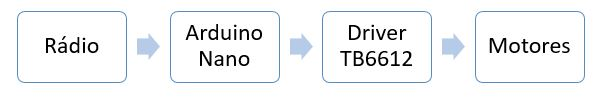
\includegraphics[scale=0.5]{esquema_robo.JPG}
        \caption{Esquema de funcionamento do robô.}
    \label{fig:esquema_robo} 
\end{figure}

Seguindo o diagrama representado na Fig. \ref{fig:esquema_robo}, os componentes do robô são: um módulo de rádio, NRF24l01, um Arduino Nano, um \textit{Driver} para motores, TB6612FNG, e micro motores DC com redução de 50:1. O funcionamento do robô se baseia na transmissão das velocidades através do rádio. Estas informações são transmitidas e armazenadas em um vetor, onde cada par de posições possui a informação de velocidade e sentido que os robôs deverão seguir. O Arduino presente em cada robô recebe as informações via rádio, e envia o equivalente em sinais de PWM para a ponte H, que aciona os motores. A Fig. \ref{fig:Exemplo do vetor de transmissão} exemplifica um vetor onde são armazenadas as informações de velocidade de cada roda de cada robô.

%Figura do funcionamento do rádio
\begin{figure}[!htb]
    \centering 
        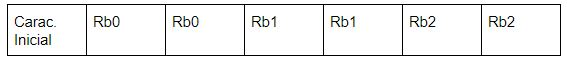
\includegraphics[scale=0.5]{vetor_radio.JPG}
        \caption{Exemplo do vetor de transmissão.}
    \label{fig:Exemplo do vetor de transmissão} 
\end{figure}

%Descrição Componentes
Rádio NRF24L01:
O módulo NRF24L01, ilustrado na Fig. \ref{fig:Radio} opera com frequência em torno de 2.4GHz (faixa de frequência e permite a configuração e construção de um canal de comunicação através da seleção de uma entre 125 frequências (canais) disponíveis, e taxa de transmissão ajustável.

\begin{figure}[!htb]
    \centering
        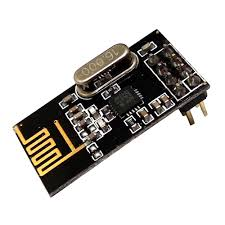
\includegraphics[scale=0.4]{radio.jpg}
        \caption{Módulo de Rádio NRF24L01.}
    \label{fig:Radio} 
\end{figure}

Ponte H (\textit{Driver}) TB6612FNG:
Havendo a necessidade de melhoria no comportamento e controle dos robôs, o \textit{Driver} TB6612FNG, ilustrado na Fig. \ref{fig:TB6612FNG} foi escolhido por melhorar a vida útil do circuito e eliminação de problemas como da força contra eletromotriz e o consumo excessivo, deteriorando precocemente as células de alimentação, impedindo seu pleno funcionamento. Robustez, tamanho reduzido e tecnologia mais atual, essa ponte H possui transistores MOSFETs permitindo atingir frequências de chaveamento em torno de 100KHz, são mais recentes e mais eficientes em relação aos modelos 
com BJTs.

\begin{figure}[!htb]
    \centering 
        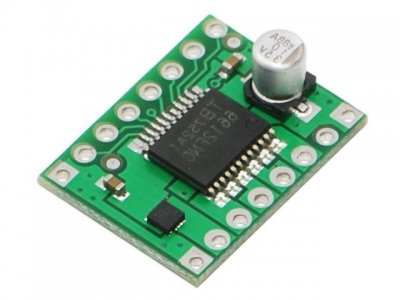
\includegraphics[scale=0.3]{TB6612FNG.jpg}
        \caption{TB6612FNG da Pololu.}
    \label{fig:TB6612FNG} 
\end{figure}

Micromotor DC:
Os motores utilizados são Micromotores DC com redução 50:1 de 6V de tensão nominal, apresentam bom torque. Visto que em versões anteriores já era utilizado e durante algumas simulações se mostrou um ótimo motor, robusto e compacto.

Bateria 18650 (4.2V):
Com grande versatilidade em sua aplicabilidade e facilidade de ser encontrada em dispositivos eletrônicos, a bateria 18650 (Fig. \ref{fig:Célula Li-ion 18650}) é uma excelente opção de alimentação ao VSS devido ao seu tamanho compatível e fidelidade na entrega de energia aos circuitos envolvendo motores com grandes quantidades de picos no consumo.

\begin{figure}[!htb]
    \centering 
        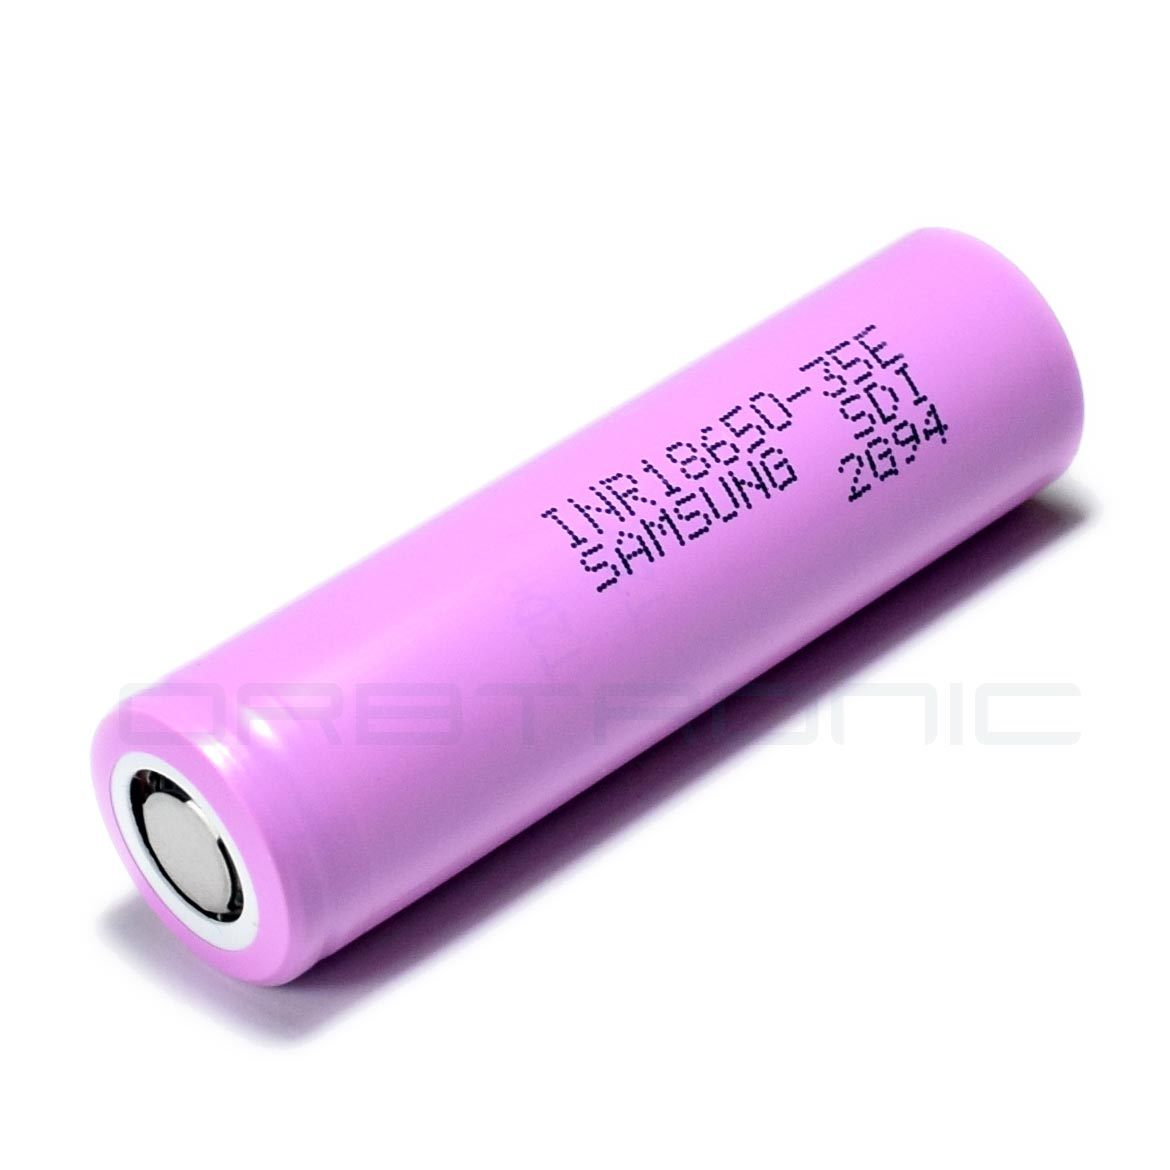
\includegraphics[scale=0.1]{bateria18650.jpg}
        \caption{Célula Li-ion 18650.}
    \label{fig:Célula Li-ion 18650} 
\end{figure}

Apesar de valor relativamente alto, compensa com sua vida útil e espaço que ocupa, se comparado com as células AA com capacidades inferiores e rápida perda no ciclo de vida útil, por conta do perfil que os robôs possuem. 
Seguindo o que foi proposto, além da utilização da bateria de Li-íon 18650, dois componentes eletrônicos foram incluídos no projeto, um módulo TP4056 (Fig. \ref{fig:Módulo Carregador TP4056}), que consiste me um circuito carregador de baterias bem pequeno e compatível com micro-USB, que possibilita uma carga segura e estável das baterias no próprio robô, além de oferecer proteção contra sobrecarga e LEDs que indicam o estado de carga das baterias. 

\begin{figure}[!htb]
    \centering
        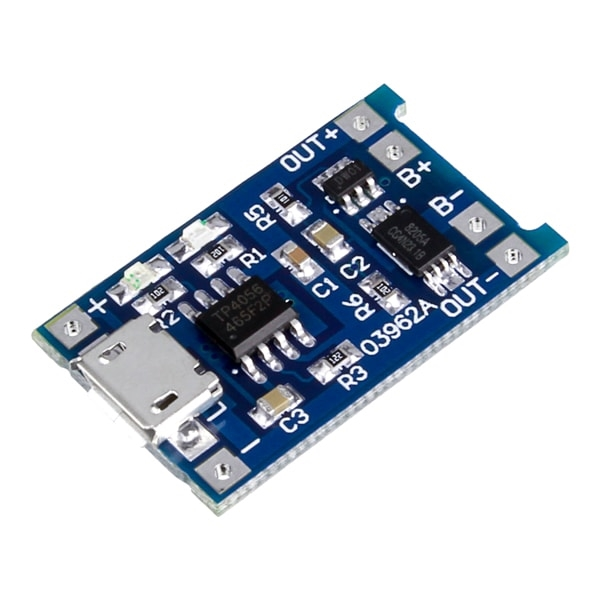
\includegraphics[scale=0.3]{TP4056.jpg}
        \caption{Módulo TP4056.}
    \label{fig:Módulo Carregador TP4056} 
\end{figure}

E um circuito regulador de tensão \textit{Step-Up} MT3608 (Fig. \ref{fig:Regulador de Tensão DC Step-Up MT3608}) também de pequenas dimensões e facilidade no uso,com eficiência de  cerca de 91, grande faixa de operação (2,5 a 28V) e saída de no máximo 2A. A aplicação de ambos no robô foi motivada pela premissa de montar um robô independente de alterações para recarga, estável, e padronizar a tensão de alimentação dos circuitos de controle (Arduino) e dos motores.

\begin{figure}[!htb]
    \centering
        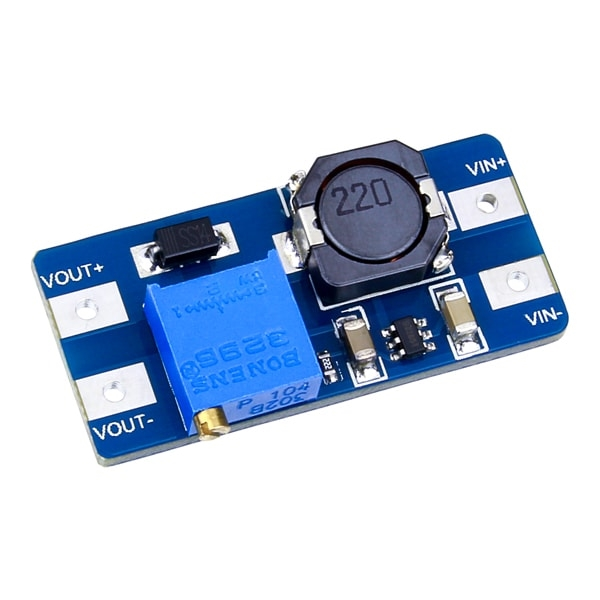
\includegraphics[scale=0.3]{mt3608.jpg}
        \caption{Regulador de Tensão DC Step-Up MT3608.}
    \label{fig:Regulador de Tensão DC Step-Up MT3608} 
\end{figure}

A rotação das rodas, e consequentemente o deslocamento do robô, são determinados por sensores ópticos TCRT5000, que codificam o movimento de dentes reflexivos fixados às rodas em pulsos enviados ao Arduino. Esses pulsos são contados e servem de realimentação ao acionamento direcionado a cada motor, permitindo a aplicação de controle de velocidade aos motores.

Do lado do computador pessoal, o envio dos comandos também ocorre através de um circuito controlado por um Arduino Nano conectado a uma interface USB. Este Arduino recebe os comandos a serem enviados aos robôs e os transmite por meio de um transceptor de rádio NRF24L01 idêntico ao utilizados nos robôs. 
%\end{document}
